\newcommand{\dk}[0]{\Delta k(t)}
\newcommand{\K}[0]{\kappa}
\newcommand{\Oc}[0]{\Omega_c}
\newcommand{\Oz}[0]{\Omega_0}
\newcommand{\Od}[0]{\Omega_d(t)}
\newcommand{\xp}[0]{x_+}
\newcommand{\xm}[0]{x_-}
\newcommand{\Op}[0]{\Omega_{+}}
\newcommand{\Om}[0]{\Omega_{-}}
\newcommand{\Opm}[0]{\Omega_{\pm}}
\newcommand{\Omp}[0]{\Omega_{\mp}}
\newcommand{\dO}[0]{\Delta\Omega}
\newcommand{\od}[0]{\omega_d(t)}
\renewcommand{\a}[0]{a(t)}
\renewcommand{\b}[0]{b(t)}
\newcommand{\odr}[0]{\omega_{drive}}
\newcommand{\ar}[0]{\overline{a}(t)}
\newcommand{\br}[0]{\overline{b}(t)}


\newpage

\section{Following the paper}

\ls \tcite{Frimmer_2014}.
\li \tcite{smith2010waves}.
\le

\begin{comment}
\begin{python}
%load_ext autoreload
%autoreload 2
%xmode Plain
# import pennylane as qml
import numpy as np
import matplotlib.pyplot as plt
from math import pi
\end{python}

\begin{result}
\end{result}
\end{comment}

\begin{center}
  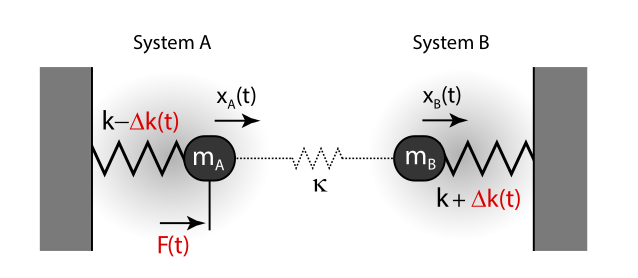
\includegraphics[width=0.6\textwidth]{img/osc.png}
\end{center}

\subsection{Motion equation}

We start by applying Newton's second law to the system. We set \(F(t) = 0\) since we are not
interested in the direct manipulations. Instead, we treat \(\Delta k\) as a function of time $\dk$
and use it to control the system by analogy to quantum control.

As usual, we assume that $x_a$ and $x_b$ are also functions $\Rat \to \Rat$ from time to coordinate.

We assume that positive forces act from left to right and negative from right to left.

\[
\begin{cases}
  \displaystyle - (k - \dk) \cdot x_a - \K (x_a - x_b) = m \ddot{x_a} \\
  \displaystyle \K(x_a - x_b) - (k + \dk) x_b = m \ddot{x_b}
\end{cases}
\]

Divide by $m$ and rearrange to get equation (1) from the paper:

\begin{equation}
  \begin{cases}
    \displaystyle \ddot{x_a} + x_a\left[\frac{k + \kappa}{m} - \frac{\dk}{m}\right] - x_b\frac{\kappa}{m} = 0 \\
    \displaystyle \ddot{x_b} + x_b\left[\frac{k + \kappa}{m} + \frac{\dk}{m}\right] - x_a\frac{\kappa}{m} = 0
  \end{cases}
\label{main}
\end{equation}


Following the paper, we define:
\ls Carrier frequency $\Oz^2 = \frac{k+\K}{m}$
\li Coupling frequency $\Oc^2 = \frac{\K}{m}$
\li Detuning frequence $\Od^2 = \frac{\dk}{m}$
\le

% We assume that \(\Oz \gg \Oc\).

In matrix form, the (\ref{main}) becomes:

\[
\ddot{\begin{bmatrix}
  x_a \\
  x_b
\end{bmatrix}}
+
\begin{bmatrix}
  \Oz^2 - \Od^2 & -\Oc^2 \\
  -\Oc^2 & \Oz^2 + \Od^2
\end{bmatrix}
\begin{bmatrix}
  x_a \\
  x_b
\end{bmatrix}
=
0
\]


\begin{GREY}
The common strategy to solve these equations in the absence of detuning $\Od$ would be to (a) get
equivalent independent eigenmode equations by adding and subtracting the equations and substituting
$\xp = x_a + x_b$ and $\xm = x_a - x_b$; (b) Solve the new equations one by one. In the paper
authors show that the detuned eigenmodes differ from the ideal case. However, they continue with the
$\xp$ and $\xm$ approach and a number of additional assumptions despite providing us with the exact
eigenmode equations.
\end{GREY}

\begin{QUESTION}
In the paper, the exact solutions for eigenfrequences are provided: \(\Opm = \left(\Oz^2
\mp \sqrt{\Od^4 + \Oc^4}\right)^{1/2}\). How to come to it?
\end{QUESTION}

\subsection{Normal modes}

In order to get to (almost) independent equations we follow the paper by putting $\xp = x_a + x_b$
and $\xm = x_a - x_b$.  Then we add and subtract equations from \ref{main} to get:


\begin{equation}
\ddot{\begin{bmatrix}
  \xp \\
  \xm
\end{bmatrix}}
+
\begin{bmatrix}
  \Oz^2 - \Oc^2 & -\Od^2 \\
  -\Od^2 & \Oz^2 + \Oc^2
\end{bmatrix}
\begin{bmatrix}
  \xp \\
  \xm
\end{bmatrix}
= 0
\label{normal}
\end{equation}


We continue with this almost-diagonal matrix. Assume the solutions of the following form:

\begin{equation}
  \begin{cases}
    x_+ = a(t)e^{i\Omega_0 t} \\
    x_- = b(t)e^{i\Omega_0 t}
  \end{cases}
  \label{sol}
\end{equation}

where $a(t)$ and $b(t)$ are complex amplitudes. We put these forms into \ref{normal}, calculate the
second derivatives and apply the following simplifications:

\ls Slowly-varying amplitude approximation (SVEA): neglect terms containing second derivatives of
$a(t)$ and $b(t)$.
\le


\[
2i
\dot{\begin{bmatrix}
  \a \\
  \b
\end{bmatrix}}
=
\begin{bmatrix}
  \displaystyle \frac{\Oc^2}{\Oz} & \displaystyle \frac{\Od^2}{\Oz} \\
  \displaystyle \frac{\Od^2}{\Oz} & \displaystyle -\frac{\Oc^2}{\Oz}
\end{bmatrix}
\begin{bmatrix}
  \a \\
  \b
\end{bmatrix}
\]

We futher note that:
\ls $\Od^2/\Oz$ is approximately equal to the $\dO = \Om - \Op$ as they are defined in the
paper, due to the known fact about the squre root
difference\footnote{\url{https://math.stackexchange.com/questions/231234/difference-of-square-roots-approximation}}.
\li Following the paper, we define rescaled detuning frequency $\od = \Od^2/\Oz$.
\le

This is how we get to the paper's equation (13) which resembles the Schrodinger equation
\(i\hbar\dot{\ket{\psi}} = H\ket{\psi}\).

\begin{equation}
i2
\dot{\begin{bmatrix}
  \a \\
  \b
\end{bmatrix}}
=
\begin{bmatrix}
  \dO & \od \\
  \od & -\dO
\end{bmatrix}
\begin{bmatrix}
  \a \\
  \b
\end{bmatrix}
\label{normalamp}
\end{equation}

\subsection{Parametrically-driven system}

We now proceed to choosing the particular $\dk$. Following the paper we put:

\[
  \dk = -2 \Oz m A * \cos(\odr t)
\]

so that

\[
  \od = -A (e^{i \odr t} + e^{-i \odr t})
\]

We apply the Rotating wave approximation (RWA):
\ls Assume
    \[
      \begin{cases}
      \displaystyle \a = \ar \exp(-i\frac{\odr}{2}t) \\
      \displaystyle \b = \br \exp(+i\frac{\odr}{2}t)
      \end{cases}
    \]
\li Neglect the $exp(\pm3i\odr t/2)$ terms as we believe they will be averaged out on our time
    scale.
\le

to get the equation (17) from the paper:


\begin{equation}
i2
\dot{\begin{bmatrix}
  \ar \\
  \br
\end{bmatrix}}
=
\begin{bmatrix}
  (\dO - \odr) & -A \\
  -A & -(\dO - \odr)
\end{bmatrix}
\begin{bmatrix}
  \ar \\
  \br
\end{bmatrix}
\label{rotamp}
\end{equation}

We may note that the main matrix of the equation does not contain functions any more. While the
paper contains the full solution (19) for these equations, we are mainly interested in running Rabi
oscillations, for which we can choose $\odr = \dO$. For this special case, the equations will show
as $2i \dot{\ar} + A \br = 0$ and $2i \dot{\br} + A \ar = 0$ with the solution
\footnote{\url{https://web.spms.ntu.edu.sg/~ydchong/teaching/05_complex_oscillations.pdf}}:

\[
  \begin{cases}
    \displaystyle \ar = a_0 \cos(\frac{A}{2}t) + i b_0 \sin(\frac{A}{2}t) \\
    \displaystyle \br = b_0 \cos(\frac{A}{2}t) + i a_0 \sin(\frac{A}{2}t)
  \end{cases}
\]

where $a_0 = \overline{a}(0)$ and $b_0 = \overline{b}(0)$.

In other words, in order to transfer the system from "$+$" eigenmode $\begin{bmatrix}a_0 \\
0\end{bmatrix}$ to "$-$" eigenmode $\begin{bmatrix}0 \\ b_0\end{bmatrix}$ one need to enable the
$\od = \dO$ detuning and wait for $\pi/A$ time units.

\section{Simulation}

\subsection{Direct simulation}
We demonstrate how one can transfer energy from one eigenmode to another using the parametric-driven
detuning. First we define the Python dataclass describing the detuned ascillator problem.

  \begin{comment}
    \begin{sh}
    printf '\\begin{%s}\n' 'python'
    cat $PROJECT_ROOT/python/mechanical_bloch.py | sedlines.sh OscProblem
    printf '\\end{%s}\n' 'python'
    \end{sh}
  \end{comment}

  %result
  \begin{python}
  @dataclass
  class OscProblem:
    m:       float = 0.9   # mass in kg
    k:       float = 5     # constant for main oscillating springs
    K:       float = 0.9   # constant for spring connecting two oscillators
    A:       float = 0.1   # amplitude of the spring constant oscillation
    sigma02: float = (k + K) / m
    sigmac2: float = K / m
    dsigma:  float = sigmac2 / sqrt(sigma02)
    wdrive:  float = dsigma
    delta:   float = dsigma - wdrive
    sigmaR:  float = sqrt(A**2 + delta**2)
  \end{python}
  %noresult


We represent the time-specific input parameters in a separate structure.

  \begin{comment}
    \begin{sh}
    printf '\\begin{%s}\n' 'python'
    cat $PROJECT_ROOT/python/mechanical_bloch.py | sedlines.sh Schedule
    printf '\\end{%s}\n' 'python'
    \end{sh}
  \end{comment}

  %result
  \begin{python}
  Time = float
  # DriveEnabled = list[tuple[Time,Time]]  # [(Start, Duration)]
  
  class Schedule:
    """ Encodes the time input parameters. """
    tspan:tuple[Time,Time]   # Overall simulation time span, (Start, Stop).
    time:ndarray             # Time points within the simulation time span.
    tcutoff:Time             # Time when we turn the drive off
  
    def __init__(self, tcutoff:Time|None=None):
      nt = 1000
      self.tspan = (0, 90)
      self.time = np.linspace(self.tspan[0], self.tspan[1], nt)
      self.tcutoff = tcutoff if tcutoff else self.tspan[1]
  \end{python}
  %noresult


We represent results of the simulation as the arrays of values encoding $x_a$, $x_b$, their
speeds and optional normal modes.


  \begin{comment}
    \begin{sh}
    printf '\\begin{%s}\n' 'python'
    cat $PROJECT_ROOT/python/mechanical_bloch.py | sedlines.sh Simulation
    printf '\\end{%s}\n' 'python'
    \end{sh}
  \end{comment}

  %result
  \begin{python}
  @dataclass
  class Simulation:
    t  :ndarray               # Time ticks
    xa :ndarray               # Positions of the 1st bob
    va :ndarray               # Velocities of the 1st bob
    xb :ndarray               # Positions of the 2nd bob
    vb :ndarray               # Velocities of the 2nd bob
    xp :ndarray|None = None   # (+)-mode coordinates
    xm :ndarray|None = None   # (-)-mode coordinates
    xpA:ndarray|None = None   # (+)-mode amplitudes
    xmA:ndarray|None = None   # (-)-mode amplitudes
    def __post_init__(self):
      if self.xp is None:
        self.xp = self.xa + self.xb
      if self.xm is None:
        self.xm = self.xa - self.xb
  \end{python}
  %noresult

We want to compare the results of the direct simulation of (\ref{main}) with the values predicted by
(\ref{sol}). The former is made using \verb|solve_ivp|.

  \begin{comment}
    \begin{sh}
    printf '\\begin{%s}\n' 'python'
    cat $PROJECT_ROOT/python/mechanical_bloch.py | sedlines.sh scheduled_coupled_detuned_oscillators
    printf '\\end{%s}\n' 'python'
    \end{sh}
  \end{comment}

  %result
  \begin{python}
  def scheduled_coupled_detuned_oscillators(p:OscProblem, s:Schedule, i:Initials)->Simulation:
    """ Solve the Coupled oscillators problem with detuning, as described in the "The Classical Bloch
    Equations" paper. Assume that detuning drive signal is enabled according to the schedule `s`.
    """
    xa0, va0, xb0, vb0 = list(i.__dict__.values())
    m, k, K, *_ = list(p.__dict__.values())
    sigma02, A = p.sigma02, p.A
    sigma0 = sqrt(sigma02)
    state0 = [xa0, va0, xb0, vb0]
  
    def _ode(t, state):
      xa, va, xb, vb = state
      dk = -2.0 * sigma0 * m * A * cos(p.wdrive * t) if t<s.tcutoff else 0.0
      dxadt = va
      dxbdt = vb
      dvadt = - xa * ((k + K) / m - dk / m) + xb * (K / m)
      dvbdt = - xb * ((k + K) / m + dk / m) + xa * (K / m)
      return [dxadt, dvadt, dxbdt, dvbdt]
  
    solution = solve_ivp(_ode, s.tspan, state0, t_eval=s.time)
    return Simulation(solution.t, *[np.array(x) for x in solution.y])
  \end{python}
  %noresult

\subsection{Comparing with theoretical solution}

The latter is calculated using Numpy directly:

  \begin{comment}
    \begin{sh}
    printf '\\begin{%s}\n' 'python'
    cat $PROJECT_ROOT/python/mechanical_bloch.py | sedlines.sh coupled_detuned_oscillator_theoretic
    printf '\\end{%s}\n' 'python'
    \end{sh}
  \end{comment}

  %result
  \begin{python}
  def coupled_detuned_oscillator_theoretic(p:OscProblem, s:Schedule, i:Initials)->Simulation:
    # Given parameters and variables (these would need to be defined elsewhere in your actual code)
    # s, i, and p variables need to be established in the actual environment
  
    def _calc(t):
      a0 = i.xa0 + i.xb0
      b0 = i.xa0 - i.xb0
      a_ = a0 * jnp.cos((p.A/2.0) * t) + 1j * b0 * jnp.sin((p.A/2.0) * t)
      b_ = b0 * jnp.cos((p.A/2.0) * t) + 1j * a0 * jnp.sin((p.A/2.0) * t)
      a = a_ * jnp.exp(-1j * (p.wdrive/2.0) * t)
      b = b_ * jnp.exp(+1j * (p.wdrive/2.0) * t)
      xp = a * jnp.exp(1j * jnp.sqrt(p.sigma02) * t)
      xm = b * jnp.exp(1j * jnp.sqrt(p.sigma02) * t)
      xa = (xp + xm) / 2
      xb = (xp - xm) / 2
      return xa, xb
      # return xa, xb
  
    jax_calc = jax.jit(_calc)
    jax_dcalc = jax.jacfwd(jax_calc)
  
    @partial(jnp.vectorize)
    def _x(t):
      return _calc(t)
  
    @partial(jnp.vectorize)
    def _v(t):
      # print('t',t.shape)
      va, vb = jax_dcalc(t)
      # print('res',va.shape, vb.shape)
      return va, vb
  
    t = s.time
    jt = jnp.array(t)
  
    # Calculate the derivatives
    xa, xb = _x(jt)
    # 'speeds' will contain the first derivatives of xp and xm with respect to t
    va, vb = _v(jt)
    # xb,vb,xp,xm = [np.zeros(3) for _ in range(4)]
    # Restoring xp and xm back
    xp = xa + xb
    xm = xa - xb
  
    return Simulation(t, xa, va, xb, vb,
                      xp=xp, xm=xm,
                      xpA=np.abs(xp), xmA=np.abs(xm))
  \end{python}
  %noresult


We create the problem instance, run the simulation and plot the normal mode coordinates.

  \begin{python}
  plt.close('all')
  from mechanical_bloch import *
  from math import pi
  p = OscProblem()
  i = Initials()
  s = Schedule()
  sim = scheduled_coupled_detuned_oscillators(p, s, i)
  sim_ref = coupled_detuned_oscillator_theoretic(p, s, i)
  fig1 = splotn("dosc", sim, sim_ref)
  \end{python}

  \begin{comment}
  \begin{result}
  \end{result}
  \end{comment}

\begin{figure}[h!]
  \centering
  \includegraphics[width=0.8\textwidth]{\linline{fig1}{img/mechanical-bloch-f1-dosc.png}}
  \caption{Normal mode: low-level simulation and the predicted amplitudes.}
  \label{fig:mechanical_bloch}
\end{figure}


\subsection{Bloch sphere trajectory}

  \begin{python}
  plt.close('all')
  from mechanical_bloch import *
  p = OscProblem()
  i = Initials()
  s = Schedule(pi/p.A)
  figB = splotb("doscB", p, s, i)
  \end{python}

  \begin{comment}
  \begin{result}
  (3, 349)
  [[0.         0.         0.         0.        ]
   [0.         0.00900889 0.01801704 0.02702374]
   [1.         0.99995942 0.99983768 0.99963479]]
  <Figure size 500x500 with 1 Axes>
  \end{result}
  \end{comment}

\begin{figure}[h!]
  \centering
  \includegraphics[width=0.6\textwidth]{\linline{figB}{img/mechanical-bloch-f1-doscB.png}}
  \caption{This is a mock description of the figure illustrating the mechanical Bloch system.}
  \label{fig:mechanical_bloch}
\end{figure}


\subsection{Delaying detuning drive signal}

  \begin{python}
  from mechanical_bloch import *
  from math import pi
  p = OscProblem()
  i = Initials()
  s = Schedule(pi/p.A)
  sim = scheduled_coupled_detuned_oscillators(p,s,i)
  fig2 = splotn("dosc2", sim)
  \end{python}

  \begin{comment}
  \begin{result}
  \end{result}
  \end{comment}

\begin{figure}[h!]
  \centering
  \includegraphics[width=0.8\textwidth]{\linline{fig2}{img/mechanical-bloch-f1-dosc2.png}}
  \caption{This is a mock description of the figure illustrating the mechanical Bloch system.}
  \label{fig:mechanical_bloch}
\end{figure}


\section{AI Discussions}

\subsection{Bloch sphere}

\begin{ai}
Can you think of any Python libraries for plotting Bloch spherese?
\end{ai}

\begin{airesult}
Yes, there are specialized libraries in Python designed to handle quantum mechanics and quantum
computing which include functionality for plotting Bloch spheres. Here are two notable ones:

\begin{itemize}
  \item \textbf{QuTiP (Quantum Toolbox in Python)}: QuTiP is a comprehensive quantum computing
library. It offers tools for simulating quantum systems, and its visualization module includes
functions for plotting Bloch spheres. You can create animated Bloch spheres and visualize quantum
states using this library.
    \vsp
    QuTiP can be installed using:
    \begin{verbatim}
    pip install qutip
    \end{verbatim}

  \item \textbf{Qiskit}: Qiskit is an open-source framework for working with quantum circuits and
executing them on quantum computers. The library provides a visualization module called
`qiskit.visualization` for a variety of purposes, including plotting Bloch vectors on Bloch spheres.
    \vsp
    Qiskit can be installed using:
    \begin{verbatim}
    pip install qiskit
    \end{verbatim}

  \vsp
\end{itemize}

Both libraries are robust and facilitate the plotting and animation of quantum states, including
Bloch spheres, in addition to providing extensive functionality for simulating and executing quantum
algorithms.
\end{airesult}


\begin{ai}
Please print me a similar program using Qutip?
\end{ai}

\begin{airesult}
Certainly! Below is an example program using the QuTiP library to plot a Bloch sphere with a random
vector:

\vsp

Make sure you have QuTiP installed in your Python environment with:
\begin{verbatim}
pip install qutip
\end{verbatim}

This code generates a random vector on the Bloch sphere and uses QuTiP's \verb|Bloch| class to
visualize
it. QuTiP's \verb|Bloch| object has functions to manipulate and display the sphere, and
\verb|add_vectors| is
used here to include the randomly generated vector. You can further customize the sphere's
appearance using additional methods and properties provided by the \verb|Bloch| class.
\end{airesult}


  \begin{python}
  plt.close("all")
  import numpy as np
  from qutip import Bloch

  # Function to generate a random vector on the sphere
  def random_bloch_vector():
      phi = np.random.uniform(0, 2 * np.pi)
      theta = np.random.uniform(0, np.pi)
      x = np.sin(theta) * np.cos(phi)
      y = np.sin(theta) * np.sin(phi)
      z = np.cos(theta)
      return x, y, z

  # Generate a random Bloch vector
  x, y, z = random_bloch_vector()

  # Set up the Bloch sphere
  b = Bloch()

  # Clear default annotations
  # b.point_marker = ['o']  # Reset to avoid default markers
  # b.point_color = []      # Clear default point colors
  # b.point_size = []       # Clear default point sizes

  # Name the sphere poles as A and B
  b.zlabel = ['$A$', '$B$']

  # Add the random vector to the Bloch sphere
  b.add_vectors([x, y, z])
  b.vector_width = 5  # Linewidth for axes

  # Plot the Bloch sphere
  b.show()

  # Save the plot to a file (optional)
  b.fig.savefig("img/bloch-example2.png")
  \end{python}

  % In this version, I've cleared default annotations by resetting the point_marker, point_color,
  % and point_size attributes to ensure only the custom annotations you added, 'A' and 'B', are
  % present.

  % In this version, I've removed the plt.savefig line as it was not needed when using QuTiP's Bloch
  % class.  Instead, the Bloch class provides its own method to save figures using b.fig.savefig.

  \begin{result}
  <Figure size 500x500 with 1 Axes>
  \end{result}

\begin{figure}[h!]
  \centering
  \includegraphics[width=0.5\textwidth]{img/bloch-example2.png}
  \caption{This is a mock description of the figure illustrating the mechanical Bloch system.}
  \label{fig:mechanical_bloch}
\end{figure}


\begin{ai}
Hi model. What is the relative phase of two complex numbers?
\end{ai}

\begin{airesult}
The \textit{relative phase} of two complex numbers \( z_1 \) and \( z_2 \) refers to the difference
between their respective phases (or arguments). For a complex number \( z = x + iy \), the phase (or
argument) \(\theta\) is given by

\[
\theta = \text{arg}(z) = \tan^{-1}\left(\frac{y}{x}\right)
\]

where \( x \) and \( y \) are the real and imaginary parts of the complex number, respectively.

\vsp

Let \( z_1 = r_1 e^{i\theta_1} \) and \( z_2 = r_2 e^{i\theta_2} \) be the polar forms of the
complex numbers, where \( r_1 \) and \( r_2 \) are the magnitudes and \( \theta_1 \) and \( \theta_2
\) are the respective phases. The relative phase \(\Delta \theta\) is then given by:

\[
\Delta \theta = \theta_2 - \theta_1
\]

\vsp

This measures how much one complex number is "rotated" relative to the other in the complex plane.
\end{airesult}


\subsection{Sympy}

\begin{ai}
Hi AI. Consider an oscillator problem: given a mass on a spring, write its complex solution for x
(the coordinate) as a Sympy function of time.
\end{ai}

\begin{airesult}
To write a complex solution for the position \( x(t) \) of a mass on a spring using SymPy, we need
to represent the solution to the harmonic oscillator problem.

The differential equation for a mass \( m \) on a spring with spring constant \( k \) is given by:

\[
m \frac{d^2x}{dt^2} + kx = 0
\]

The general complex solution to this harmonic oscillator problem can be written as:

\[
x(t) = A e^{i\omega t} + B e^{-i\omega t}
\]

where \( A \) and \( B \) are constants determined by initial conditions, and \(\omega =
\sqrt{\frac{k}{m}}\) is the angular frequency.

\vsp

Let's write this solution as a function of time using SymPy:

\begin{python}
import sympy as sp

# Define the symbols
t = sp.symbols('t', real=True)
A, B = sp.symbols('A B', complex=True)
omega = sp.symbols('omega', real=True, positive=True)

# Define the complex solution for x(t)
x_t = A * sp.exp(sp.I * omega * t) + B * sp.exp(-sp.I * omega * t)

# Display the solution
x_t
\end{python}

This code will create a SymPy expression representing the complex solution \( x(t) \) for the mass
on a spring system.
\end{airesult}

\begin{python}
import sympy as sp

# Define the symbols
t = sp.symbols('t', real=True)
A, B = sp.symbols('A B', complex=True)
omega = sp.symbols('omega', real=True, positive=True)

# Define the complex solution for x(t)
x_t = A * sp.exp(sp.I * omega * t) + B * sp.exp(-sp.I * omega * t)

# Display the solution
x_t
\end{python}

\begin{result}
A*exp(I*omega*t) + B*exp(-I*omega*t)
\end{result}


\begin{ai}
Great! Now please use Sympy to calculate the time-derivative of x to get the equation for speed.
\end{ai}

\begin{airesult}
To calculate the time derivative of \( x(t) \) to find the velocity (or speed) of the mass on the
spring, we can use SymPy's differentiation capabilities. The velocity \( v(t) \) is the first
derivative of the position \( x(t) \) with respect to time \( t \).

\vsp

Here's how you can do it in SymPy:

\begin{python}
# Calculate the derivative of x_t with respect to time t
v_t = sp.diff(x_t, t)

# Display the velocity equation
v_t
\end{python}

The resulting expression \( v(t) \) will give you the velocity of the mass as a function of time:

\[
v(t) = \frac{dx}{dt} = i\omega A e^{i\omega t} - i\omega B e^{-i\omega t}
\]

This velocity equation reflects the time rate of change of the position \( x(t) \).
\end{airesult}

\begin{python}
# Calculate the derivative of x_t with respect to time t
v_t = sp.diff(x_t, t)

# Display the velocity equation
v_t
\end{python}

\begin{result}
I*A*omega*exp(I*omega*t) - I*B*omega*exp(-I*omega*t)
\end{result}


\begin{ai}
Great! Now lest define $x_0$ and $v_0$ and use Sympy to calculate formulas for $A$ and $B$ from
these values!
\end{ai}

\begin{airesult}
To find expressions for the constants \( A \) and \( B \) in terms of the initial conditions \( x_0
\) (initial position) and \( v_0 \) (initial velocity), we can set up a system of equations. These
conditions are:

\[
x(0) = x_0 = A + B
\]

\[
v(0) = v_0 = i\omega A - i\omega B
\]

\vsp

We can solve these equations using SymPy to express \( A \) and \( B \) in terms of \( x_0 \) and \(
v_0 \):

\begin{python}
# Define initial conditions
x_0, v_0 = sp.symbols('x_0 v_0', real=True)

# Create equations from initial conditions
eq1 = sp.Eq(A + B, x_0)
eq2 = sp.Eq(sp.I * omega * A - sp.I * omega * B, v_0)

# Solve for A and B
solutions = sp.solve((eq1, eq2), (A, B))

# Display solutions for A and B
solutions
\end{python}

The solution will provide the expressions for \( A \) and \( B \) in terms of \( x_0 \) and \( v_0
\):

\[
A = \frac{x_0}{2} + \frac{v_0}{2i\omega}
\]

\[
B = \frac{x_0}{2} - \frac{v_0}{2i\omega}
\]

These expressions allow you to determine the constants \( A \) and \( B \) given the initial
conditions of the system.
\end{airesult}

\begin{python}
# Define initial conditions
x_0, v_0 = sp.symbols('x_0 v_0', real=True)

# Create equations from initial conditions
eq1 = sp.Eq(A + B, x_0)
eq2 = sp.Eq(sp.I * omega * A - sp.I * omega * B, v_0)

# Solve for A and B
solutions = sp.solve((eq1, eq2), (A, B))

# Display solutions for A and B
solutions
\end{python}

\begin{result}
{A: (omega*x_0 - I*v_0)/(2*omega), B: (omega*x_0 + I*v_0)/(2*omega)}
\end{result}
